\documentclass[twocolumn]{article}
\usepackage{blindtext}
\usepackage{hyperref}
\usepackage{graphicx}
\usepackage{float}
\usepackage{framed}
\usepackage[style=ieee]{biblatex}
\addbibresource{sample.bib}

\title{Customer Segmentation Clustering based on Demographics and Behaviors}
\author{Spencer Hirsch}
\date{\today}


\begin{document}

% In place of Homework 4, the instructions for the Project 2 report will be changed. The report is required to be written like an academic paper. A minimal outline is:

% - An abstract summarizing your work in <350 words
% - An introduction section with discussion of at least 5 published papers related to your efforts
% - A methods section discussing your preprocessing and models
% - A results section discussing your experiments, model tuning, and performance comparison of models you used
% - A conclusion including your main findings

\twocolumn[
\begin{@twocolumnfalse}

\maketitle
\begin{framed}
\noindent\textbf{Abstract:} Identifying similaries between customers can be a useful strategy for companies when creating marketing campaigns. By analyzing the 
demographics and the purchasing behaviors of customers, a company can gain better insight into their customer base.
With valuable insight there is potential to release marketing campaigns targeted towards these groups to increase sales.
By employing unsupervised machine learning we can better identify the characteristics of similar groups to aid in
such campaigns. This study aims to utilize customer demographic and purchasing behaviors to identify trends and group consumers
together based on these characteristics. Through the use of three different unsupervised machine learning clustering methods 
we can identify groups with shared characteristics and attempt to optimize these groups with a variety of preprocessing and 
feature reduction methods to increase the effectiveness of these models in an attempt to find the most effective model for this
study.
\end{framed}

\centering
\textbf{\textit{Keywords -- Machine learning; customer segmentation; clustering algorithm}}

\vspace{\baselineskip}
\end{@twocolumnfalse}
]


\section{Introduction}

Customer segmentation can be a powerful technique used by retailers in order to gain a better understanding of their target markets. For a business to be sucessful they must be able to cater towards their customer base, and address their specific needs. In the modern world, machine learning techniques can be utilized to make it easier for companies to better understand their customers. Customer segmentation can be used to break a larger group of people into smaller groups, separatiing them based on their shared characteristics, such as, income or how much an individual spents on wine. This information can be especially useful for marketing strategies as companies would be able to share special benefits with these groups of people to draw them in.

The data used for this exploration can be seen in Table 1, all data refers strictly to their demographic information or their shopping behaviors.\cite{patel} This dataset was not explicitly stated to be from any sort of market or company, however, it is fair to assume that the data was collected from some sort of grocery store. This seems to be the case for all features, the only feature that seems to be odd for a grocery store is the "Amount spent on gold products". Nonetheless, the other features appear to refer to a grocery store, therefore for the purpose of this study that is what we will assume.

\subsection{Related Work}

Customer segmentation can serve as a useful tool in many disciplines, Zhao dicusses a handful of potential uses when it comes to the application of customer segmentation. Whether it be for marketing purposes as previously mentioned but also for exploration purposes. Zhao brings up the possibility of utilizing this tool to determine new markets to enter.\cite{zhao} This could be an incredibly useful tool for a company looking to expand the scope of their business. If a company idenities trends in their data indication that the market is starting to lean a specific direction, they would be able to tailor their products or services to meet this demand. Zhao's discussion of customer segmentation doesn't necessarily focus on strictly unsupervised machine learning methods, the article discusses two methods, recency, frequency, and monetary (RFM) and K-Mean clustering algorithms.\cite{zhao} Rather than performing an exploration into the methods the article provides a general overview of the field at the time of publishing.

Rather that exploring potential methods of customer segmentation, Holy and Sokol bring customer segmentation into the real-world. Their study deals with the study and development of a clustering algorithm to be utilized by a major Czech drugstore chain.\cite{sokol} Holy and Sokol utilize a variety of clustering methods paried with K-Means in order to better understand the patterns of customers, RFM, as discussed in Zhao,\cite{zhao} purchased products structure (PPS), and store mission (SM).

Similarly to the study that I have conducted here, John, Shobayo, and Ogunleye aim to study a variety of unsupervised machine learning methods, along with Principle Component Analysis and RFM.\cite{john} The goal of the study is similar to mine, as they are aiming to find the most effective method for customer segmentation. The authors of this paper explore, K-Means clustering, Gaussian mixture model (GMM), density-based spatial clustering of applications with noise (DBSCAN), agglomerative clustering, and balanced iterative reduction and clustering using hierarchies (BIRCH).\cite{john} The study proved to perform well with the authors being able to acheieve a Silhoutette Score, a measure of consistency in the cluster, of 0.8, through the use of PCA and GMM.\cite{john}

Just as the previous study, Hicham and Karim utilize a number of unsupervised machine learning models for the purposes of customer segmentation. Their paper proposes a clustering ensemble method of, DBSCAN, K-Means, Mini Batch K-Means, and MeanShift. Through the use of their method, they were able to acheive a Silhouette Score of 0.73.\cite{hicham} This method proved to be useful, DBSCAN itself was only able to acheive 0.72 itself, so there was marginal gain with their technique.\cite{hicham}

Turkmen also performs a study using a variety of methods in hopes of acheving greater results, in their paper they weight K-means clustering, hierarchical clustering, DBSCAN, and RFM.\cite{turkmen} The results of this study were not as great as the previous study using an ensemble method, Turkmen was able to acheive a Silhouette Score of 0.6 using the K-Means clustering algorithm.\cite{turkmen} 

We can see that there have been numerous efforts and resources dedicated to studying the use of a variety of clustering methods for the purpose of customer segmentation. In the following study, we will see the reoccurence of clustering methods, such as, K-Means clustering, Hierarchical clustering, and DBSCAN clustering as well as the introduction of new preprocessing methods that were not used in the above studies.

\begin{table*}
    \centering
        \begin{tabular}{|c|c|}
            \hline
            \textbf{Feature Name} & \textbf{Feature Description} \\
            \hline
            Id & Unique customer identifier. \\
            Year\_Birth & Birth year of customer. \\
            Education & Highest level of education obtained by customer. \\
            Marital\_Status & Marital status of customer. \\
            Income & Annual income of customer. \\
            Kidhome & Number of young children in the home. \\
            Teenhome & Number of teenagers in the home. \\
            Dt\_Customer & Date when customer first enrolled. \\
            Recency & Last visit of customer. \\
            MntWines & Amount spent on wines. \\
            MntFruits & Amount spent on fruits. \\
            MntMeatProducts & Amount spent on meats. \\
            MntFishProducts & Amount spent on fish. \\
            MntSweetProducts & Amount spent on sweets. \\
            MntGoldProds & Amount spent on gold products. \\
            NumDealsPurchases & Number of purchases made as part of a discount promotion. \\
            NumWebPurchases & Number of purchases made through website. \\
            NumCatalogPurchases & Number of purchases made through catalog \\
            NumStorePurchases & Number of purchases made in store. \\
            NumWebVisitsMonth & Number of times customer has visited the website. \\
            \hline
        \end{tabular}
    \caption{Original columns in dataset after removal of marketing campaign information.}
\end{table*}

\section{Methods}

Three methods of unsupervised machine learning cluserting methods were used, K-Means Clustering, Hierarchical Clustering, and DBSCAN. In addition to these three methods a variety of preprocessing methods and feature reduction methods were used to reduce the dimensionality of the data. The goal of course to find the best combination of methods that provide the most efficient model. Just as John, Shobayo, and Ogunleye\cite{john}, Hicham and Karim\cite{hicham}, and Turkmen\cite{turkmen}, the primary metric used in determing the sucess of the models was the Silhouette Score. This value helps us determine how well the clustering methods is constructing the clusters. A Silhouette Score closer to 1 signifies that the clusters are more closely associated, whereas a score close to -1 means that they are not.

Once accessing the dataset, we start by manually preprocessing the data, this includes removing some of the features in the dataset as well modifying categorical features of the dataset. Once this was complete, preprocessing using a variety of algorithms was employed, as well as feature reduction algorithms. Once this was complete, the three clustering models where employed and underwent hyper-parameter tuning to find the optimal number of clusters for the highest Silhouette Score.


\subsection{Preprocessing}

In order to prepare the data for this exploration, it was necessary to clean up the data to adhere to the task at hand.
Due to the nature of the project it was fitting that marketing campaign was removed from the dataset, the initial dataset contained five marketing campaigns as well as response information from the customers. For the prupose of clustering based on demographic and behaviors this information was not necessarily important.
 
In addition to this feature removal, much of the existing data in the dataset was categorical, rather than leaving objects
in the dataframe, the data was converted to contain only numeric values, this process included 1-hot encoding all categorical
data and splitting the datetime object into three new features, month, day, and year. Following the manual deletion and modification of the original dataset, the new dataset consisted of 33 features.

After manual feature reduction and cleaning was performed, additional preprocessing was done on the data. This included utilizing
a variety of methods: Standard Scaler, Robust Scaler, Quantile Transformation, and Log Transformation. All of these methods were used 
in an attempt to increase the effectiveness of the clusters. We can see that some of the preprocessing methods formed stonger clusters than others. Robust Scaler, seen in figure two, was the worst preprocessing method used when it came to clustering. The method that had the strongest clustering was the preprocessing performed with Quantile Transformation, seen in Figure 3.

\begin{figure}
    \centering
    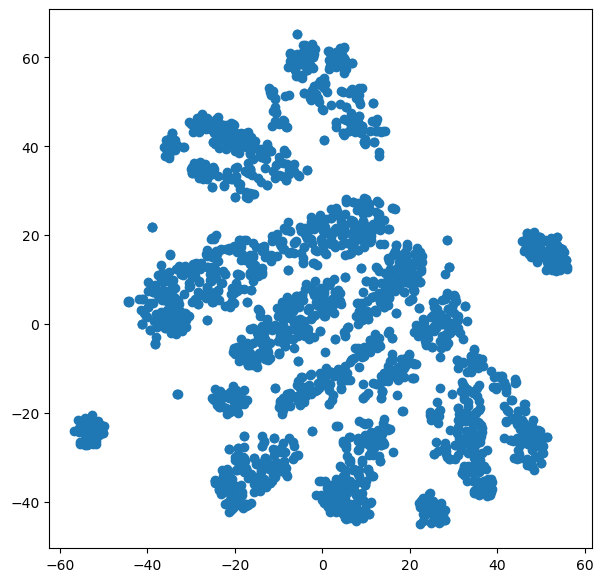
\includegraphics[width=0.4\textwidth]{images/standard_scaler.png}
    \caption{Visual representation of data preprocessed using Standard Scaler.}
\end{figure}

In Figure 1, we can see well forming clusters, that appear to spread out more in a pedal shape. This is not a necessarily poor way to cluster the data, however this method was not as effective as clustering as some of the others.

\begin{figure}
    \centering
    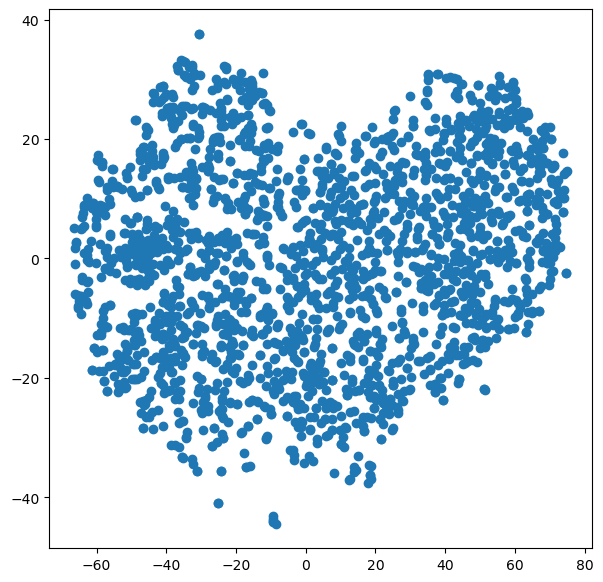
\includegraphics[width=0.4\textwidth]{images/robust_scaler.png}
    \caption{Visual representation of data preprocessed using Robust Scaler.}
\end{figure}

Figure 2 contains the cluster for the worst performing preprocessing method, creating seemingly one complete cluster rather than the other preprocessing methods which created smaller more effective clusters.

% \vspace{-1.7cm}
\begin{figure}
    \centering
    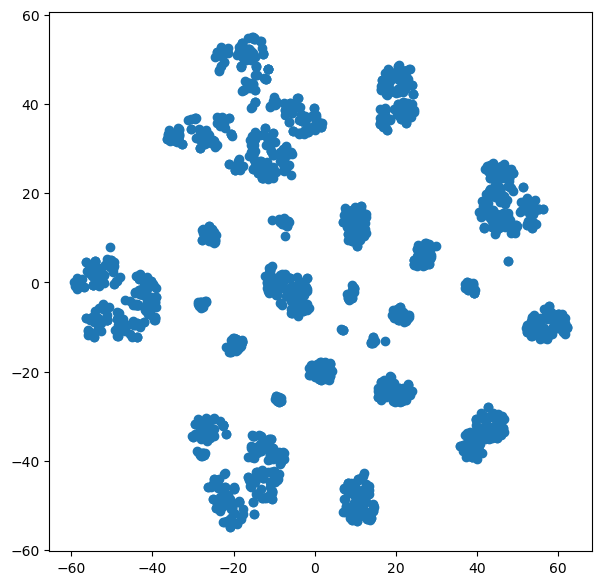
\includegraphics[width=0.4\textwidth]{images/quantile_transform.png}
    \caption{Visual representation of data preprocessed using Quantile Transformation.}
\end{figure}

Figure 3 created what appears to be the most effective method at preprocessing for this dataset, Quantile Transfomation. Creating much smaller and more compact cluster compared to the other methods.

Lastly, Log Transformation, performed similarly to how the Standard Scaler preprocessing performed. It created smaller clusters within a larger cluster of data. 

\begin{figure}
    \centering
    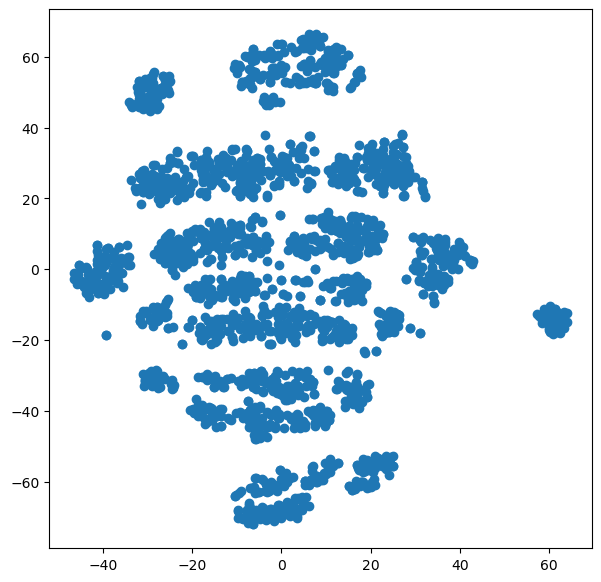
\includegraphics[width=0.4\textwidth]{images/log_transformed.png}
    \caption{Visual representation of data preprocessed using Log Transformation.}
\end{figure}


\subsection{Feature Reduction}

Feature reduction was a necessary addition to this project, with the preprocessed dataset contain 33 features. Two feature reduction were tested to determine which method would be most effective. PCA was the first method tested and the results were very poor. Which led to the discovery of the T-distributed Stochastic Neighbor Embedding (t-SNE) method. This method turned out to be far more effective for this dataset. Figure 5 depicts the t-SNE feature reduction with the n\_clusters parameter set to 2. This was the most effective feature reduction method. Additional n\_cluster values were tested, n\_clusers set to 3 is shown in Figure 6. We can see that the clustering was far less effective using this method. For this reason the only feature reduction used going forward is the t-SNE method with n\_clusers set to 2, this is used acorss all methods discussed below.

\begin{figure}
    \centering
    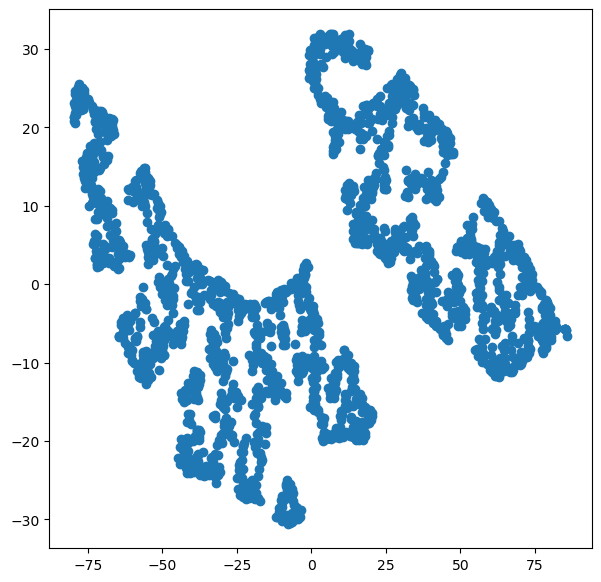
\includegraphics[width=0.4\textwidth]{images/tsne_2.png}
    \caption{Visual representation of data with t-SNE feature reduction with 2 n\_clusters.}
\end{figure}



\begin{figure}
    \centering
    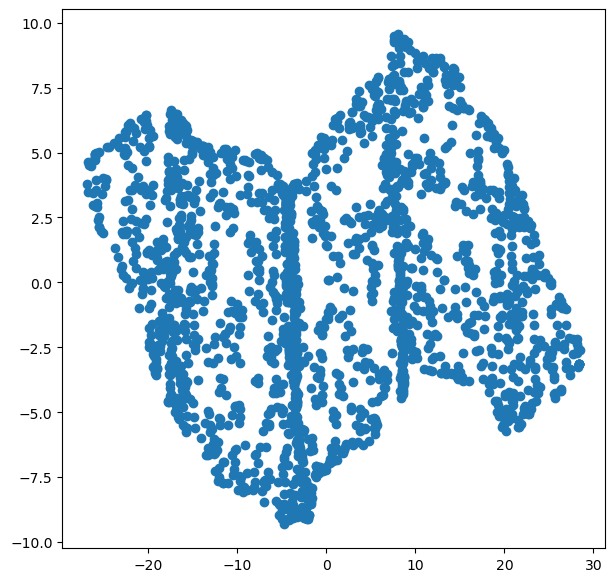
\includegraphics[width=0.4\textwidth]{images/tsne_3.png}
    \caption{Visual representation of data with t-SNE feature reduction with 3 n\_clusters.}
\end{figure}

\subsection{Clustering}

For the purposes of this study three unsupervised machine learning clustering algorithms were employed, K-Means, Hierarchical, and DBSCAN. As previously mention, the metric that determines the highest performing method is the Silhouette Score. 

\subsubsection{K-Means}

\begin{figure}
    \centering
    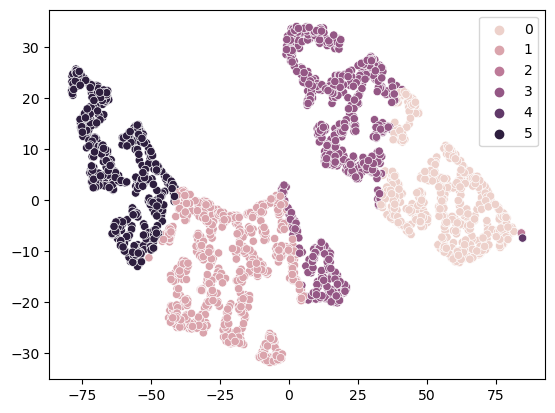
\includegraphics[width=0.4\textwidth]{images/kmeans.png}
    \caption{Visual representation of dataset clustered with K-Means method with t-SNE feature reduction applied.}
\end{figure}

The first method tested was the K-Means algorithm, this was paired with all of the previously mentioned preprocessing methods, however, with K-Means none of these methods proved to be useful. K-Means clustering paired with t-SNE was sufficient in acheiving the highest Silhouette Score for this method. K-Means unwent hyper-parameter tuning where I attempted to optimize the Silhouette Score my increasing the number of clusters, for this case 2 cluster throuhg 10 clusters where tested. K-Means with six clusters ended up being the best performing model. This acheived a Silhouette Score of 0.3843, in comparison to the other methods discussed later in this paper this was the worst performing model. Figure 6, visualizes the results returned using K-Means clustering. We can see that there were farily well constructed clusters for 4 of them, however we can see some outliers towards the right hand side of the data. There are two individual points that seemingly construct their own clusters. Upon this realization, the assumption would have been that four clusters would perform better, this however, was not the case. A common theme shared among all results of K-Means was that these points created their own clusters, with the expection of the 2 cluster model.

\subsubsection{Hierarchical}

\begin{figure}
    \centering
    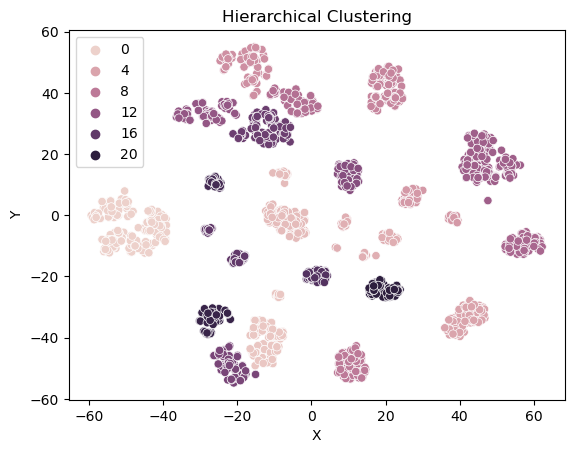
\includegraphics[width=0.4\textwidth]{images/hierarchical.png}
    \caption{Visual representation of dataset clustered with Hierarchical method with t-SNE feature reduction and Quantile Transformation applied.}
\end{figure}

Hierarchical clustering was another method that was used for this project, similarly to K-Means, t-SNE feature reduction was used to reduce the dimensionality of the data. However, in addition to t-SNE the dataset was preprocessed using Quantile Transformation. All preprocesing methods were used, however, the highest Silhouette Score was returned using this method paired with t-SNE. This turned out to be the best performing model, with a Silhouette Score of 0.6483. We can see the resulting cluster visualzation in Figure 8, we can see how vastly different the results are in comparison to the K-Means Clustering algorithm. The cluster were much smaller and more concise which allowed for the higher Silhouette Score.


\subsubsection{DBSCAN}

\begin{figure}
    \centering
    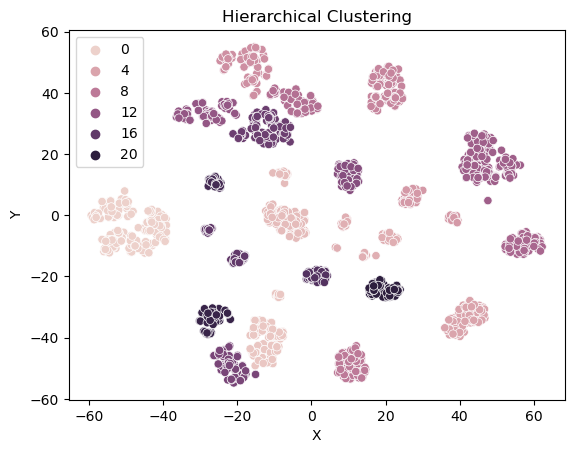
\includegraphics[width=0.4\textwidth]{images/hierarchical.png}
    \caption{Visual representation of dataset clustered with DBSCAN method with t-SNE feature reduction and Quantile Transformation applied.}
\end{figure}

Just as shown with Hierarchical Clustering, DBSCAN was used in part with t-SNE and Quantile Transfomation preprocessing. Again, all preprocesing methods were used for this model, however these returned the highest Silhouette Score. DBSCAN was not as effective as Hierarchical Clustering, however it was the second best performing method wiht a Silhouette Score of 0.5785. The visualization of the clusters can be seen in Figure 9, the clustering appears to be very similar to that of Figure 8, this is because the preprocesing method and feature reduction method used in both DBSCAN and Hierarchical Clustering were the same. This means that the results were solely reliant on the clustering algorithms themselves. Just as with the two previos model, DBSCAN went through hyper-parameter tuning in an attempt to increase the effectiveness of the model.

\section{Results}

It is clear that Hierarchical Clusering paired with t-SNE and Quantile Transformation was the most effective model at grouping customers together. With these clusters now, we can view the related information for these groups, to idenitfy patterns in this data to see what these groups are like. Tables, 2, 3, and 4 refer to selected clusters from the Hierachical clustering model. The cluster consists of 21 clusters, all looking similar to the ones presented. With these selected clusters distinct patterns can be indentified. We can see that one cluster has a significatly higher income than the others, and have fewer discounted purchases. In addition to these two attributes, we see and increase in the amount spent on wines. Information such as this is especially useful to companies who are interested in learning more about their customers and their spending habits. For example, Cluster 1 from Table 2, has the highest number of discounted purchases. This could be evidence that additional coupons would draw these customers in more, therefore we could look further at their purchasing history to better cater coupons to these groups to bring in more of their business.

\begin{table}
    \centering
    \textbf{Hieracical Clustering: Cluster 1}
        \begin{tabular}{|c|c|}
            \hline
            \textbf{Feature Name} & \textbf{Cluster Average} \\
            \hline
            Annual Income & \$49,770.84 \\
            Amount Meat & \$44.22 \\
            Amount Wines & \$82.01 \\
            Discount Purchases & 3 \\
            Store Purchases & 4 \\
            Web Purchases & 3 \\
            \hline
        \end{tabular}
    \caption{Extracted average information from Cluster 1 of Hierachical Clustering paired with t-SNE feature reduction and Qunatile Transfomation.}
\end{table}

\begin{table}
    \centering
    \textbf{Hieracical Clustering: Cluster 4}
        \begin{tabular}{|c|c|}
            \hline
            \textbf{Feature Name} & \textbf{Cluster Average} \\
            \hline
            Annual Income & \$56,041.42 \\
            Amount Meat & \$171.61 \\
            Amount Wines & \$394.30 \\
            Discount Purchases & 2 \\
            Store Purchases & 6 \\
            Web Purchases & 4 \\
            \hline
        \end{tabular}
    \caption{Extracted average information from Cluster 4 of Hierachical Clustering paired with t-SNE feature reduction and Qunatile Transfomation.}
\end{table}

\begin{table}
    \centering
    \textbf{Hieracical Clustering: Cluster 19}
        \begin{tabular}{|c|c|}
            \hline
            \textbf{Feature Name} & \textbf{Cluster Average} \\
            \hline
            Annual Income & \$74,421.19 \\
            Amount Meat & \$472.14 \\
            Amount Wines & \$557.78 \\
            Discount Purchases & 1 \\
            Store Purchases & 8 \\
            Web Purchases & 5 \\
            \hline
        \end{tabular}
    \caption{Extracted average information from Cluster 19 of Hierachical Clustering paired with t-SNE feature reduction and Qunatile Transfomation.}
\end{table}

\section{Conclusion and Future Work}

This paper studied the effectiveness of a variety of preprocessing, feature reduction, and unsupervised machine learning methods in an attempt to find the most effective model for customer segmentation. Utilizing unsupervised machine learning for customer segmentation has proven itself to be a useful tool. Unfortunately, this study was unable to acheive as significant results as some mentioned in the Related Works section, such as Hicham and Karim's study.\cite{hicham} However, acheiving a Silhouette Score of 0.65 was not too far off. After reading Hicham and Karim's work, it would be interesting to follow their approach in creating an ensemble method with my selected models to attemptd to increase the Silhouette Score. Another interesting addition would be using this model on another customer segmentation dataset and to observe its performance. Overall, the study proved to be effective at clustering customers based on their demographic information and purchasing behaviors.


\twocolumn[
\begin{@twocolumnfalse}
\printbibliography
\end{@twocolumnfalse}
]


\end{document}